\begin{figure}
    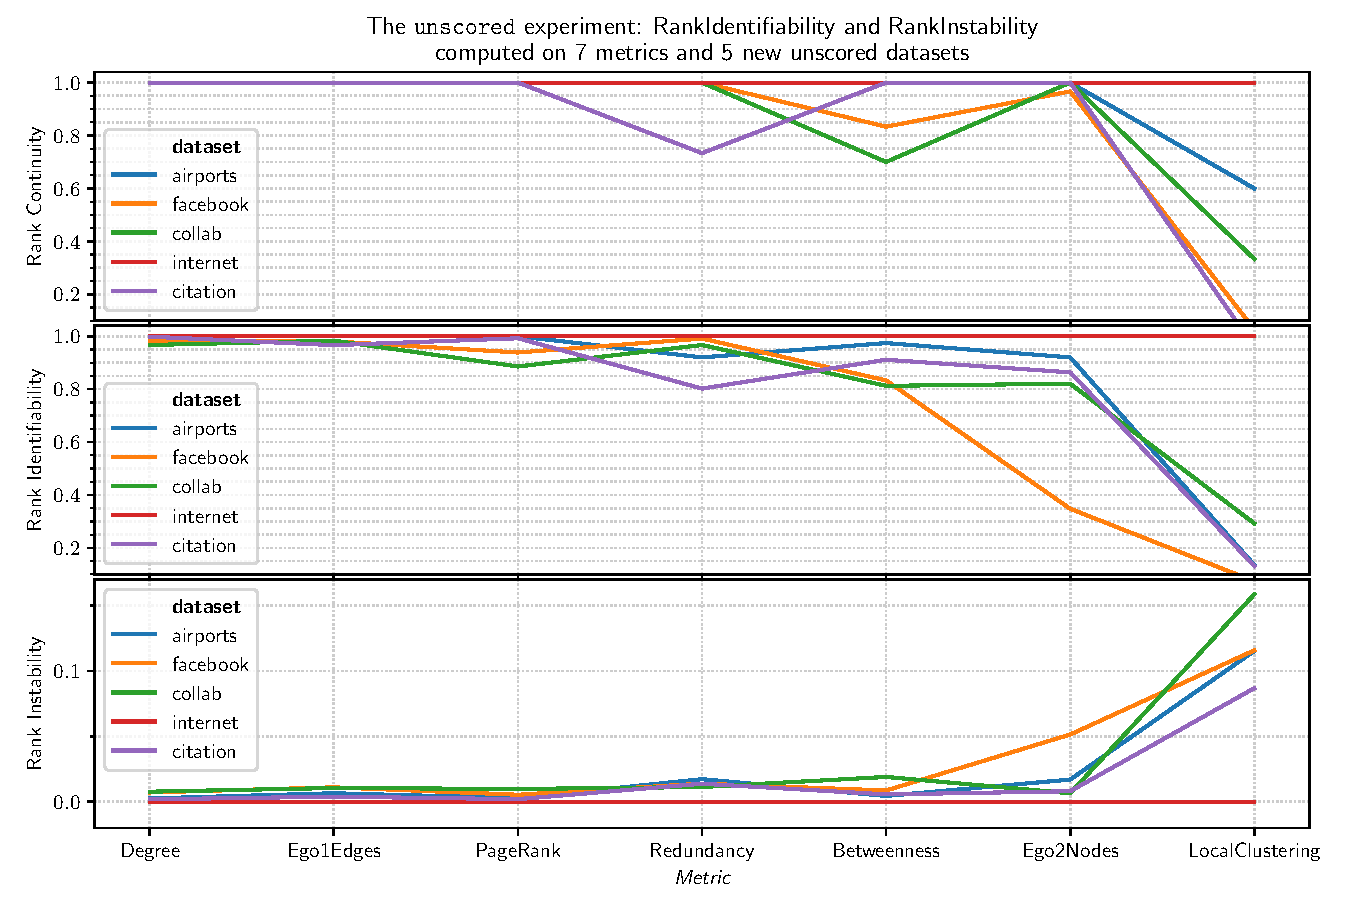
\includegraphics[width=\linewidth]{plot_unscored.pdf}
    \vspace*{-0.6cm}
    \caption{Evaluating RankIdentifiability and RankInstability on 5 new unscored datasets, generating graphs by randomly deleting $4\%$ of edges.}
    \label{fig:plot_unscored}
    \footnotesize
    \begin{flushleft}
        High values of RankIdentifiability mean high \textsl{robustness}, whereas high values of RankInstability mean low \textsl{robustness}.
        Metrics are sorted from left to right by their decreasing combined robustness.
    \end{flushleft}
\end{figure}
